\documentclass[12pt, border=8pt]{standalone}
\usepackage{tikz}
\usepackage{amsmath, amssymb, bm}
\usepackage{xcolor}
\usetikzlibrary{positioning, arrows.meta, calc, fit, backgrounds}

\begin{document}


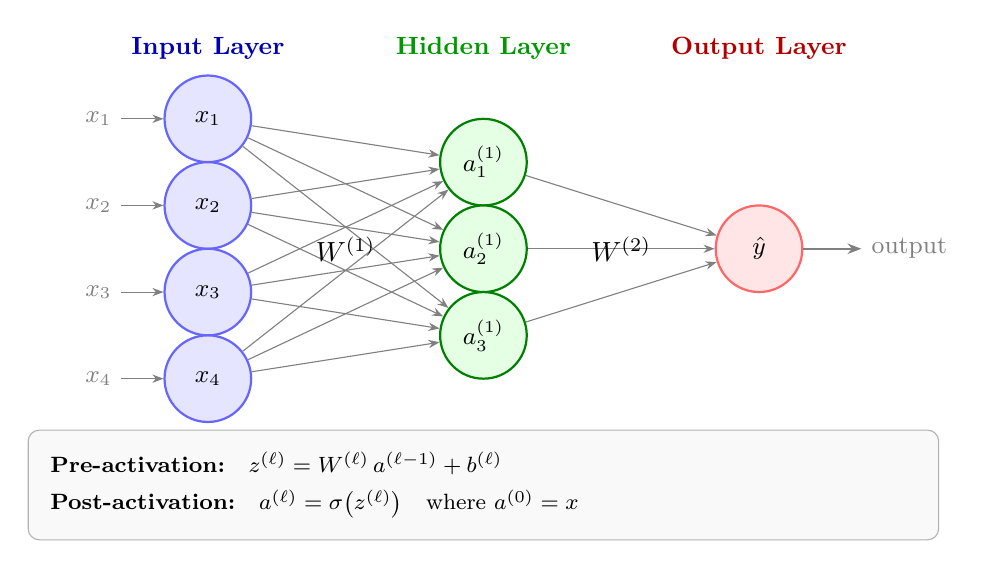
\begin{tikzpicture}[
  inputnode/.style={circle, draw=blue!60, fill=blue!10, thick, minimum size=1.1cm, font=\small},
  hiddennode/.style={circle, draw=green!50!black, fill=green!10, thick, minimum size=1.1cm, font=\small},
  outputnode/.style={circle, draw=red!60, fill=red!10, thick, minimum size=1.1cm, font=\small},
  conn/.style={-{Stealth[length=4pt]}, gray, thin},
  inarrow/.style={-{Stealth[length=4pt]}, gray, thin},
  outarrow/.style={-{Stealth[length=5pt]}, gray},
]

%% ── Input nodes ──────────────────────────────────────────────────────────────
\node[inputnode] (x1) at (0, 3.3) {$x_1$};
\node[inputnode] (x2) at (0, 2.2) {$x_2$};
\node[inputnode] (x3) at (0, 1.1) {$x_3$};
\node[inputnode] (x4) at (0, 0.0) {$x_4$};

%% ── Hidden nodes ─────────────────────────────────────────────────────────────
\node[hiddennode] (a1) at (3.5, 2.75) {$a_1^{(1)}$};
\node[hiddennode] (a2) at (3.5, 1.65) {$a_2^{(1)}$};
\node[hiddennode] (a3) at (3.5, 0.55) {$a_3^{(1)}$};

%% ── Output node ──────────────────────────────────────────────────────────────
\node[outputnode] (yhat) at (7.0, 1.65) {$\hat{y}$};

%% ── Input arrows from left ───────────────────────────────────────────────────
\foreach \i in {1,2,3,4} {
  \draw[inarrow] ($(x\i)+(-1.1,0)$) node[left, font=\small] {$x_\i$} -- (x\i);
}

%% ── Input → Hidden connections ───────────────────────────────────────────────
\foreach \src in {x1,x2,x3,x4} {
  \foreach \dst in {a1,a2,a3} {
    \draw[conn] (\src) -- (\dst);
  }
}

%% ── Hidden → Output connections ──────────────────────────────────────────────
\foreach \src in {a1,a2,a3} {
  \draw[conn] (\src) -- (yhat);
}

%% ── Output arrow to right ────────────────────────────────────────────────────
\draw[outarrow, thick] (yhat) -- ++(1.3,0) node[right, font=\small] {output};

%% ── Weight labels ────────────────────────────────────────────────────────────
\node[font=\normalsize] at (1.75, 1.65) {$W^{(1)}$};
\node[font=\normalsize] at (5.25, 1.65) {$W^{(2)}$};

%% ── Layer title labels ───────────────────────────────────────────────────────
\node[font=\bfseries\small, blue!70!black]  at (0,   4.2) {Input Layer};
\node[font=\bfseries\small, green!60!black] at (3.5, 4.2) {Hidden Layer};
\node[font=\bfseries\small, red!70!black]   at (7.0, 4.2) {Output Layer};

%% ── Annotation box ───────────────────────────────────────────────────────────
\node[
  draw=gray!60, rounded corners=4pt, fill=gray!5,
  text width=11cm, align=left, font=\footnotesize,
  inner sep=8pt
] at (3.5, -1.35) {%
  \textbf{Pre-activation:}\quad
    $z^{(\ell)} = W^{(\ell)}\,a^{(\ell-1)} + b^{(\ell)}$\\[4pt]
  \textbf{Post-activation:}\quad
    $a^{(\ell)} = \sigma\!\left(z^{(\ell)}\right)$\quad
    where $a^{(0)} = x$
};

\end{tikzpicture}

\end{document}
